\graphicspath{{img/model/out}{img/model}}

\chapter{Physical Model}
In this chapter, we will introduce the physical model that will be used in this thesis. We will start by introducing the 1D TASEP, which is a well-studied model for transport processes. Then, we will introduce the 2D TASEP, which is the model that we will use in this thesis. Finally, we will introduce the concept of smarticles, which are smart particles that use reinforcement learning to maximize transport in the 2D TASEP.

\section{1D TASEP}
\label{sec:1d-tasep}
The TASEP is one of the most well-studied models in non-equilibrium statistical physics. It can be used as a stochastic model for transport processes on a 1D lattice and was first introduced by MacDonald, Gibbs and Pipkin in 1968 \cite{macdonald_kinetics_1968} as a model for protein synthesis, where particles are ribosomes and sites are codons. It was later introduced in mathematics by Spitzer in 1970 \cite{spitzer_interaction_1970}. The name TASEP stands for \textit{totally asymmetric simple exclusion process}. \textit{Totally asymmetric} means that particles can only move in one direction. In the more general ASEP, particles have different rates $p$ and $q$ for jumping to the left or right respectively. \textit{Simple} means that particles can only move to the next site. \textit{Exclusion} means that each site can only be occupied by one particle. \textit{Process} means that the model is a stochastic process, specifically a continuous-time Markov process on the finite state space
\begin{equation}
    \mathcal{S} = \{0, 1\}^L \text{,}
    \label{eq:state-space}
\end{equation}
where $L$ is the number of sites. Each site can either be occupied by a particle or empty, so the state space consists of all possible configurations of particles on the lattice. It can be treated as a continuous-time process, as each particle moves according to its own internal clock, although in this thesis we will discretize time by picking a random particle in each time step.


The 1D TASEP can be treated with periodic boundary conditions, where the first and last sites are connected as shown in figure \ref{fig:tasep_1d_periodic}, or with different rates for insertion and removal of particles, as shown in figure \ref{fig:tasep_1d_finite}. Exact solutions are known for the one-dimensional TASEP and different phases can be found, depending on these rates or the density of particles \cite{schutz_exact_1997,blythe_nonequilibrium_2007}.

\begin{figure}[h]
    \centering
    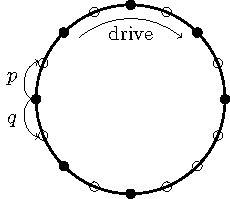
\includegraphics[width=0.55\textwidth]{tasep_a.pdf}
    \caption{A 1D ASEP with periodic boundary conditions. The number of particles is constant. Each particle has a probability $p$ to move clockwise and a probability $1-p$ to move counterclockwise. If the target site is occupied, the particle stays. If $p=1$ and $q=0$, the process is totally asymmetric (TASEP).}
    \label{fig:tasep_1d_periodic}
\end{figure}

\begin{figure}[h]
    \centering
    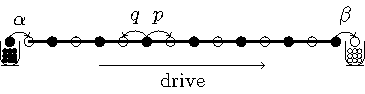
\includegraphics[width=0.75\textwidth]{tasep_b.pdf}
    \caption{A 1D finite TASEP. The reservoir on the left inserts particles with rate $\alpha$ and the reservoir on the right removes particles with rate $\beta$.}
    \label{fig:tasep_1d_finite}
\end{figure}



\section{2D TASEP}
\label{sec:2d-tasep}
The TASEP can be generalized to higher dimensions. In this thesis, we will use the 2D TASEP, which can be used as a simplified model for traffic flow with multiple lanes or intracellular transport processes, for example the movement of motor proteins on microtubules. In this case, the process is totally asymmetric in one direction and symmetric in the other direction. Particles can only move to the right (\enquote{forward}), up or down. We will use periodic boundary conditions in both directions, which means that the number of particles is constant, like on a torus. A small 8x4 version of the 2D TASEP is shown in figure \ref{fig:tasep_2d}. The 2D TASEP is not as well studied as the 1D TASEP. No exact solutions are known and only approximations, such as mean-field theory, exist \cite{goykolov_asymmetric_2007}.
\\
\begin{figure}[h]
    \centering
    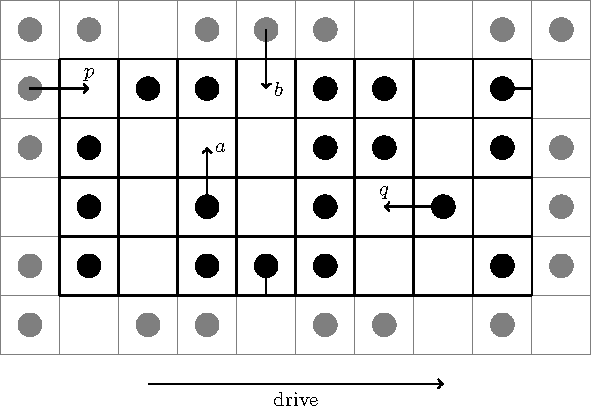
\includegraphics[width=0.8\textwidth]{tasep_2d.pdf}
    \caption{A 2D ASEP with periodic boundary conditions. The number of particles is constant. Each particle has a probability $p$ to move forward, a probability $q$ to move backward and probabilities $a$ and $b$ to move up or down respectively. If the target site is occupied, the particle stays. The hopping probabilities should be chosen such that $p+q+a+b=1$.}
    \label{fig:tasep_2d}
\end{figure}
In this thesis, we will increase the complexity of the 2D TASEP by introducing velocities. The velocity is implemented as a probability $v$ of actually performing an attempted jump. For example, if a particle's velocity is $v=0.5$, it will only move in 50\% of the cases where a jump is attempted and the target site is empty. For a particle with velocity $v$, the new transition rate thus becomes $p_{\text{new}} = p \cdot v$. 


After a basic numerical treatment of the classical 2D TASEP, we will try to optimize the total transport in these systems by introducing \textit{smarticles}. 

\section{Smarticles}
\label{sec:smarticles}
Smarticles (\textbf{Smart} Part\textbf{icles}) are a form of active matter as described in section \ref{sec:intelligent-matter}. In this thesis, we will use smarticles to optimize the transport in the 2D TASEP and observe how global structures can emerge from local interactions. The smarticles will be implemented as particles with a neural network that decides where to move based on the surroundings. 


This can be framed as a reinforcement learning problem, where the reward structure is defined by the goal of the system, which is to maximize transport along the drive direction. Local interactions can also be integrated into the reward structure in order to bias the learned behavior towards certain global structures.  